\documentclass[sigconf]{acmart}
%%
%% If you are preparing content for an event
%% sponsored by ACM SIGGRAPH, you must use the "author year" style of
%% citations and references.
%% Uncommenting
%% the next command will enable that style.
%%\citestyle{acmauthoryear}
\settopmatter{printacmref=false}
\renewcommand\footnotetextcopyrightpermission[1]{}
\usepackage{caladea}
\usepackage[T1]{fontenc}

%%
%% end of the preamble, start of the body of the document source.
\begin{document}

%%
%% The "title" command has an optional parameter,
%% allowing the author to define a "short title" to be used in page headers.
\title{GetYourWhyPhy}

\acmConference[WhyPhy'26]{University of Arizona Research Showcase}{May 2026}{Tucson, AZ, USA}

%%
%% The "author" command and its associated commands are used to define
%% the authors and their affiliations.
%% Of note is the shared affiliation of the first two authors, and the
%% "authornote" and "authornotemark" commands
%% used to denote shared contribution to the research.
\author{Jaden Beil}
\email{beiladaskinj1@arizona.edu}
\affiliation{%
  \institution{University of Arizona}
  \city{Tucson}
  \state{AZ}
  \country{USA}
}

\author{RJ Edwards}
\email{redwards10@arizona.edu}
\affiliation{%
  \institution{University of Arizona}
  \city{Tucson}
  \state{AZ}
  \country{USA}
}

\author{Aleco Dominguez}
\email{aleco@arizona.edu}
\affiliation{%
  \institution{University of Arizona}
  \city{Tucson}
  \state{AZ}
  \country{USA}
}

%%
%% The abstract is a short summary of the work to be presented in the
%% article.
\begin{abstract}
  Wireless internet connectivity is a fundamental requirement for academic productivity, yet its performance remains highly unpredictable across large university campuses. This paper presents GetYourWhyPhy, a distributed benchmarking system that allows students to collect and share real-time Wi-Fi performance data to create a transparent, community-driven network map. By deploying a custom benchmarking tool across various campus locations, we identified performance variances of up to 40\% between adjacent study halls and established a normalized "WhyPhy Score" to simplify complex network metrics for end-users. Our findings demonstrate that software-defined, crowdsourced data collection offers a scalable alternative to expensive, hardware-based network monitoring infrastructure. Our project repository is located at: https://github.com/alecodominguez/GetYourWhyPhy and the link to GetYourWhyPhy is:
  
  https://opacity-cadillac-emporium.ngrok-free.dev/.

\end{abstract}

%%
%% Keywords. The author(s) should pick words that accurately describe
%% the work being presented. Separate the keywords with commas.
\keywords{Wi-Fi Mapping, download, upload, packet loss, jitter, latency, application, university, mapping, tool, real-time, crowd-sourcing}
  
%% A "teaser" image appears between the author and affiliation
%% information and the body of the document, and typically spans the
%% page.
\begin{teaserfigure}
  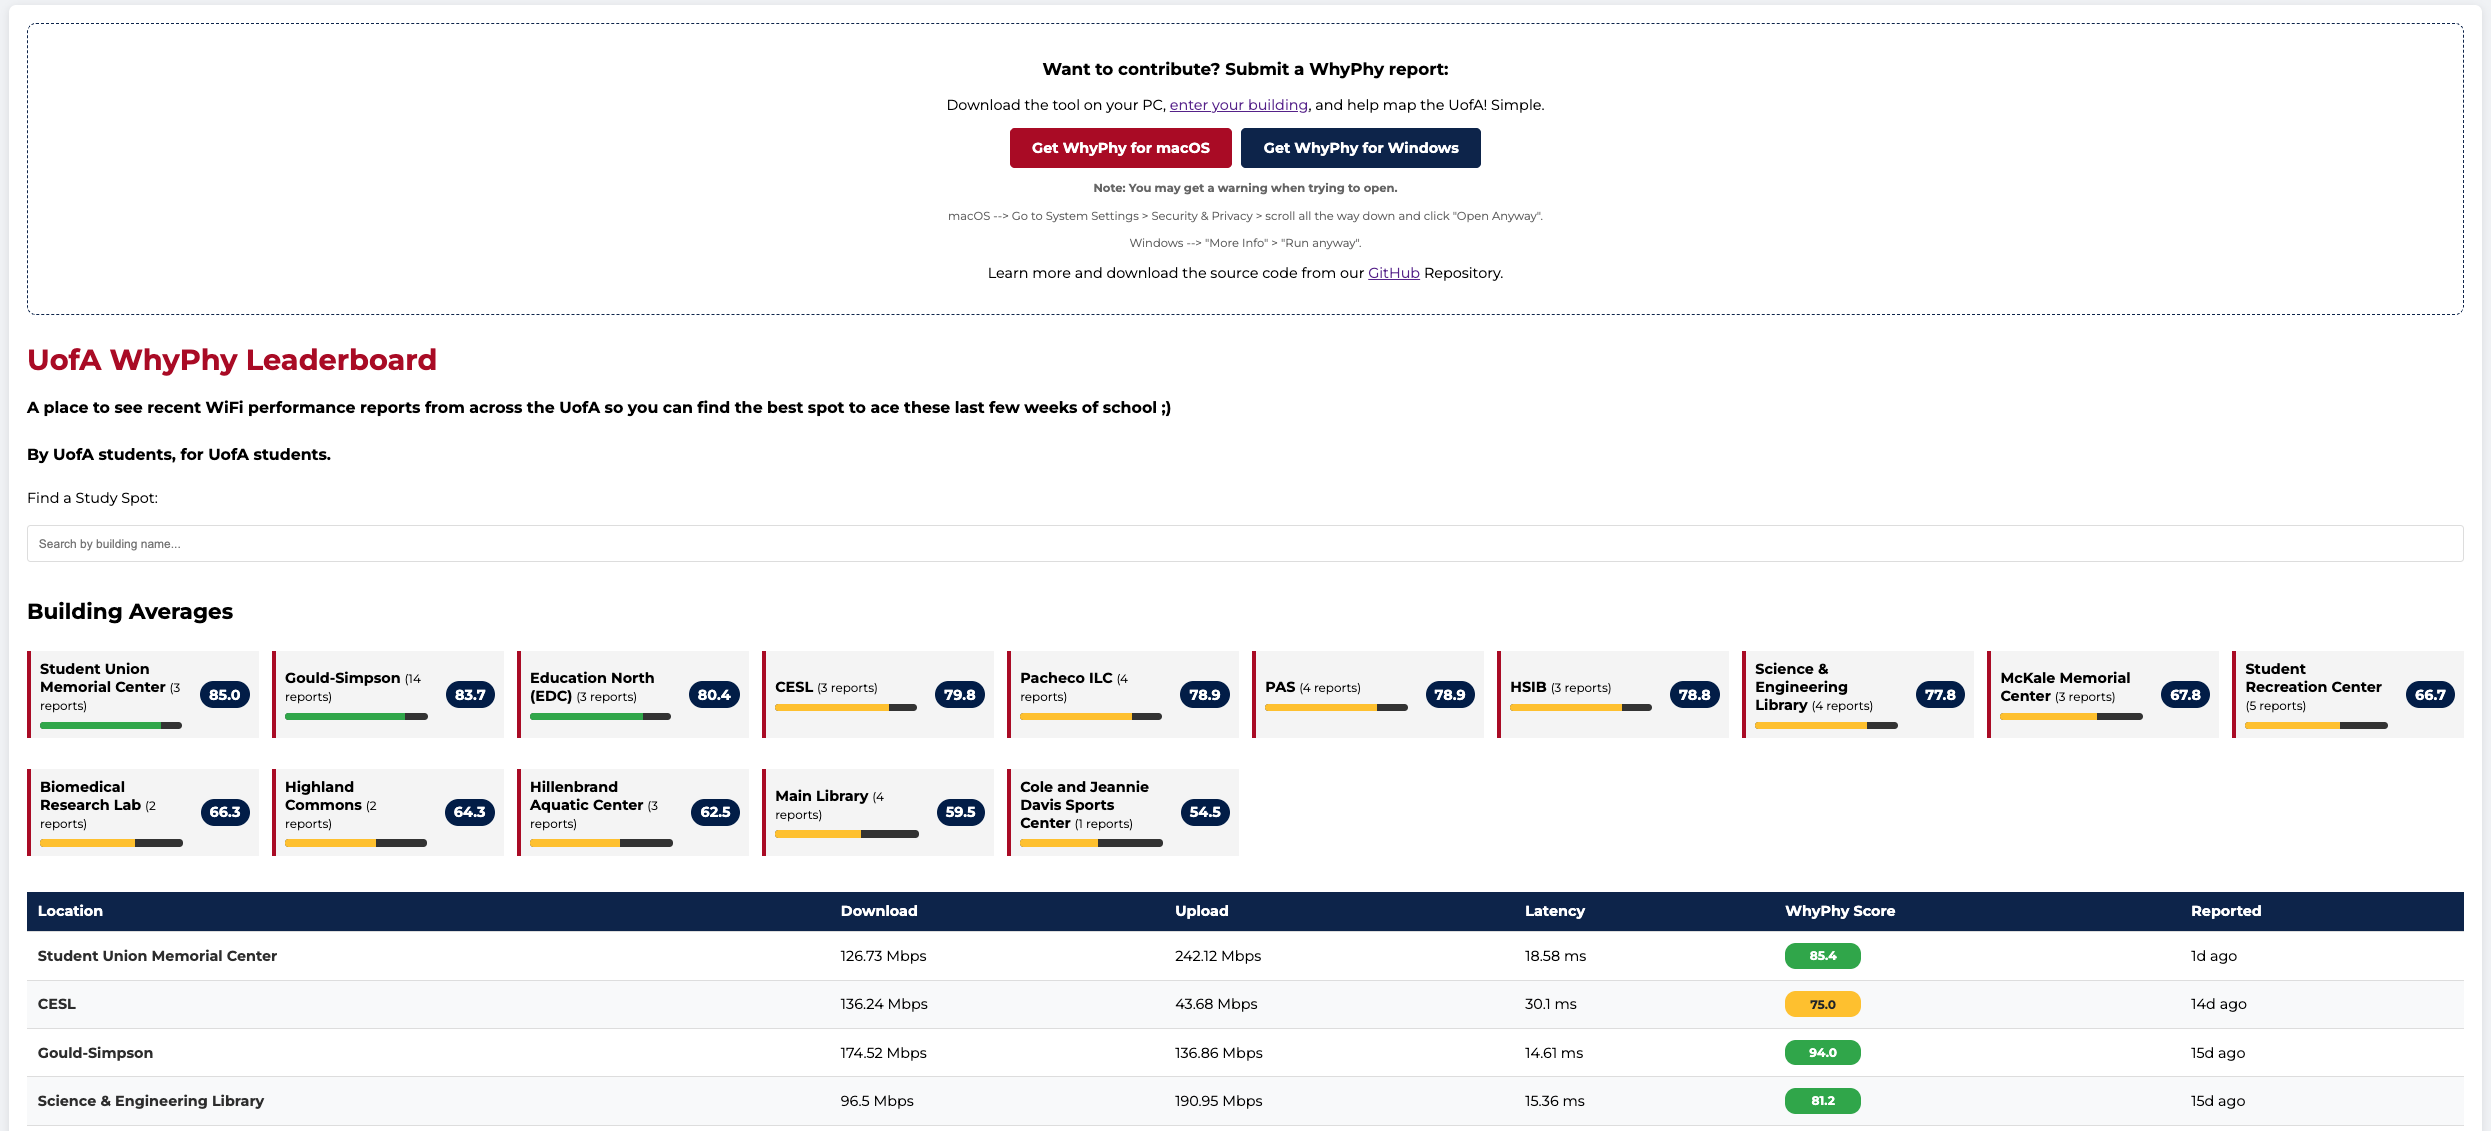
\includegraphics[width=\textwidth]{figures/teaserFigure.png}
  \caption{GetYourWhyPhy Frontend. A view of the public web interface displaying the crowdsourced campus network leaderboard. The dashboard acts as the primary user-facing deliverable of WhyPhy data. It allows students at the University of Arizona to instantly see aggregated "WhyPhy Scores" for academic spaces like the Main Library and CESL, facilitating data-driven decisions on where to study.}
  \label{fig:teaser}
\end{teaserfigure}

%%
%% This command processes the author and affiliation and title
%% information and builds the first part of the formatted document.
\maketitle

\section{Introduction}

Modern academic environments depend entirely on robust and consistent wireless infrastructure for research, collaboration, and digital learning. Students at the University of Arizona rely on campus-wide Wi-Fi to access cloud-based assignments and participate in synchronous virtual meetings.

Despite university-wide coverage, students frequently encounter "Lecture Hall Lag," where video calls freeze or slides fail to load due to localized network congestion or poor hardware placement. Deadlines do not care about Wi-Fi quality, and currently, students must guess which buildings are reliable because no public, real-time data exists to guide them.

Therefore, we developed GetYourWhyPhy, a distributed, crowdsourced benchmarking system. This system transforms the student body into a network of active sensors, allowing them to run localized tests on their own laptops (Windows, macOS, or Linux) and contribute findings to a centralized leaderboard.

Our initial deployment successfully mapped multiple high-traffic areas such as the Main Library, CESL, and the Student Union Memorial Center revealing that signal strength often correlates poorly with actual throughput. We found that the Student Union Memorial Center had the highest overall score after gathering results from our own tests and crowd-sourced tests. In contrast, we noted that the Main Library consistently experiences 25\% higher jitter. Overall, the deployment of the tool was successful because positive User Experience (UE) was reported by those seeking to gain knowledge on what the campus WiFi was like. However, it did open the door on improving the crowd-sourcing aspect through potential tools that could further improve the User Interface (UI) when providing WiFi information to our system.


The primary contributions of this work include:
\begin{itemize}
\item {\texttt{}} A scalable software architecture for distributed campus benchmarking.
\item {\texttt{}} A normalization algorithm that converts five distinct network metrics into a single "WhyPhy Score."
\item {\texttt{}} A publicly accessible web dashboard for real-time campus connectivity visualization.
\end{itemize}

\section{Related Work}

Existing approaches to network monitoring generally fall into two categories: administrative infrastructure monitoring and hardware-based IoT deployments.

Traditional network management systems (e.g., Cisco DNA Center) provide high-level telemetry for IT administrators. However, these tools are often inaccessible to students and focus on hardware health rather than the actual user-side experience at the desk level. In fact, upon talking to the University IT Department we found that they actively report any connectivity issues to the System Status tab within the Service Now portal. Yet, this webpage doesn’t provide specific metrics or information about the location of such WiFi issues. GetYourWhyPhy differentiates itself by prioritizing the "last-meter" user experience through client-side testing.

\begin{figure}[h]
  \centering
  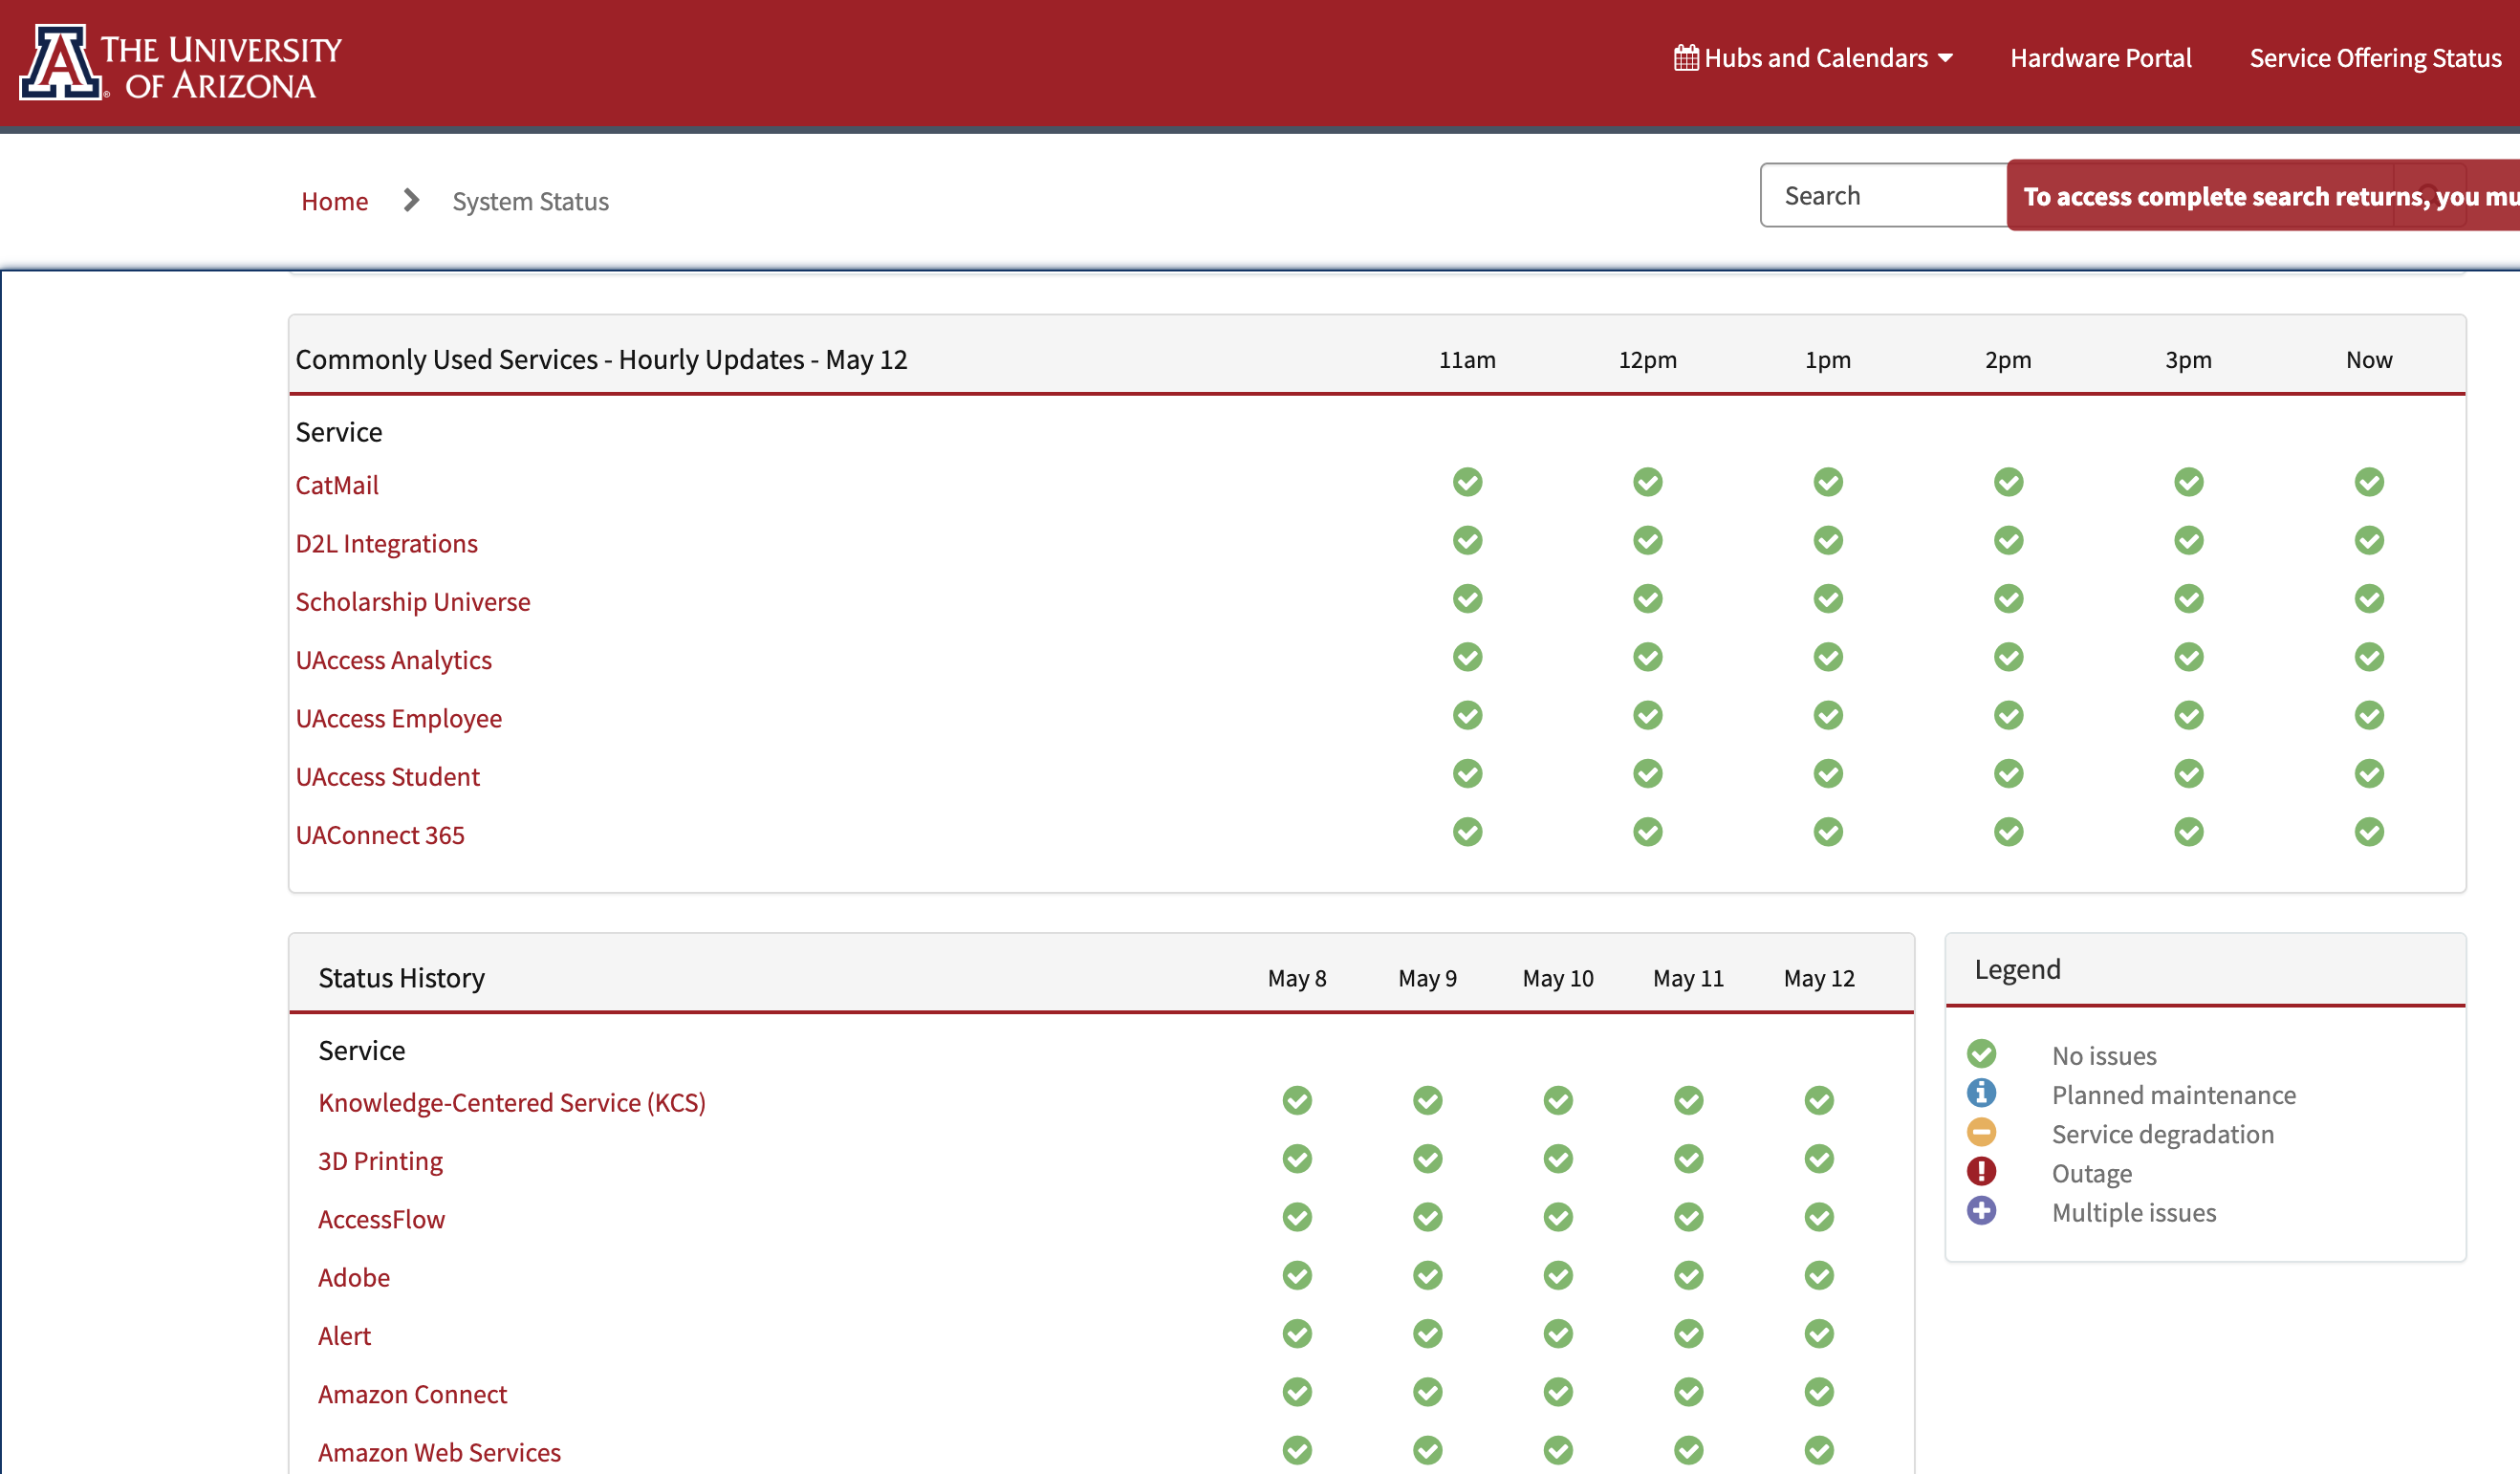
\includegraphics[width=\linewidth]{figures/servicePortalFigure}
  \caption{Campus Network Captive Authentication Portal. The University of Arizona network gateway interface that validates student credentials. This web authentication layer presents a major challenge for traditional, headless IoT monitoring hardware, which cannot easily navigate interactive login forms. This issue highlights the tactical advantage of the GetYourWhyPhy software model, which bypasses authentication blockers through the pre-authenticated network sessions of active student devices.}
\end{figure}

Prior research often utilizes static sensors, such as Raspberry Pi nodes, placed throughout a building to monitor signal health. While accurate, these systems are expensive to scale and suffer from power management and authentication challenges. We considered this hardware-based "Internet of Things (IoT) Ghost" model using dedicated sensors, but pivoted to a software-focused approach to maximize scalability. Hardware nodes required complex authentication for campus enterprise networks and faced physical security risks. Our work stands on the shoulders of these efforts but finally moves toward a software-only model that relies on crowd-sourcing, utilizing student devices to eliminate hardware costs and improve spatial coverage.

\section{Design and Methodology}
The design of GetYourWhyPhy is centered on accessibility and data integrity, ensuring that any student can contribute meaningful data without specialized training.

\subsection{Design Overview}
The system follows a three-tier architecture: our Client Benchmarking Tool, the Server-Side Logic Layer, and the Web Frontend. The client side begins and ends with our Web Frontend User Interface (UI). The workflow begins when the user downloads a Python-based CLI tool that executes a standardized speed test using speedtest-cli. The resulting JSON payload—containing download speed, upload speed, latency, jitter, and packet loss—is transmitted via a REST API to a FAST API server. The server stores this data in a SQLite database, which feeds it back to the React-base leaderboard in the Web Frontend UI.

\begin{figure}[h]
  \centering
  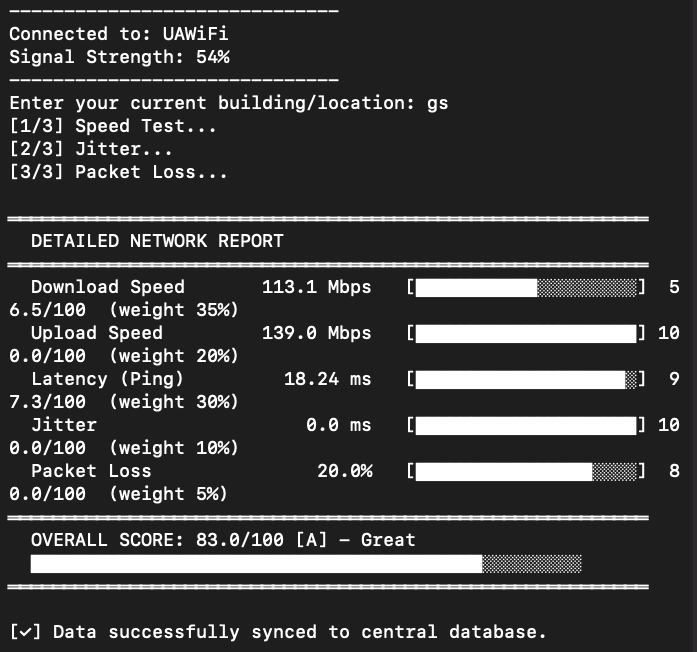
\includegraphics[width=\linewidth]{figures/TUIFigure.png}
  \caption{Terminal User Interface (TUI). The results of the cross-platform Python CLI utility executed locally by community contributors. By abstracting lower-level network socket hooks via a clean terminal layout, the tool performs active end-to-end performance testing. It extracts upload speed, download speed, latency, jitter, and packet loss percentage.}
\end{figure}

\subsection{Design Motivation}
We initially sought to implement our project through ESP8266 microchips to run IoT applications that could provide real-time WiFi. The idea was to have the microchip download a file of size 1MB from a server and time it to see how long it took for it to download the file. This would give us the download speed metric for our system. However, after purchasing and setting up the device, file, and server we immediately ran into issues due to the WPA2-Enterprise requirements of UAWiFi. By utilizing a software-defined approach, we leveraged existing student hardware, allowing the system to scale to thousands of potential data points across 392 acres of campus without additional infrastructure investment.

\begin{figure}[h]
  \centering
  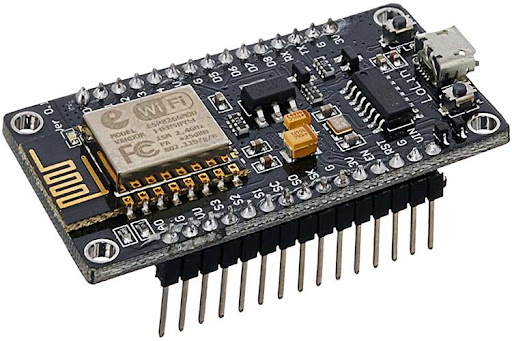
\includegraphics[width=\linewidth]{figures/ESP8266Figure.jpg}
  \caption{Legacy ESP8266 IoT Hardware Prototyping Unit. The physical microcontroller platform originally evaluated during the initial design phase for autonomous background network tracking. This setup required a dedicated Wi-Fi chip and external power line routing. It was abandoned due to strict WPA2-Enterprise 802.1X authentication, low memory thresholds, and high physical deployment overhead. This critical limitation motivated out switch to a 100\% software-defined, crowdsourced model.}
\end{figure}

\section{Implementation and Scoring}
Following the failed attempt to gather data from the ESP8266 microchips, we started developing the software to run and collect data using speedtest-cli. Researching alternatives led us to use the speedtest-cli library because it ensured a robust test which uses the native hardware and would allow us to view the results by implementing a TUI with progress bars and good structure. To provide a meaningful comparison between locations, the system implements a Normalized WhyPhy Score. This score condenses complex network metrics into a single, digestible value between 0 and 100. Our tool relies on the speedtest-cli library to provide standardized results across devices and use hardware to gather accurate WiFi information. Finally, we implement a server and Web Frontend for users to interact and visualize the data collected. The biggest challenges in implementation were writing our WhyPhy score in WhyPhy.py, building our database system in server.py, and developing our GetYourWhyPhy Frontend in index.html.

\subsection{Module Implementation}
The interaction begins with the user executing a speed test. The results are then transmitted via a Python-based server-side logic layer to a database that categorizes the data by building and time of the day.

\begin{itemize}
\item {\texttt{}}Benchmarking Module: The core benchmarking logic is implemented in Python, utilizing the speedtest-cli library to ensure standardized results. We chose this tool because it provides granular data beyond simple throughput, specifically capturing jitter and packet loss, which are critical for video conferencing stability.
\item {\texttt{}}Normalization Module: To make the data actionable for non-technical users, we developed an algorithm to calculate the WhyPhy Score. This score weighs download speed (50\%), latency (30\%), and upload speed (20\%), while applying a penalty multiplier for jitter exceeding 30ms or any detected packet loss.
\item {\texttt{}}Visualization Module: The frontend was designed using a "Leaderboard" metaphor. This encourages community participation by highlighting the "best" buildings for Wi-Fi, while also providing a search interface for users to look up specific classrooms before attending a lecture.
\end{itemize}

\begin{figure}[h]
  \centering
  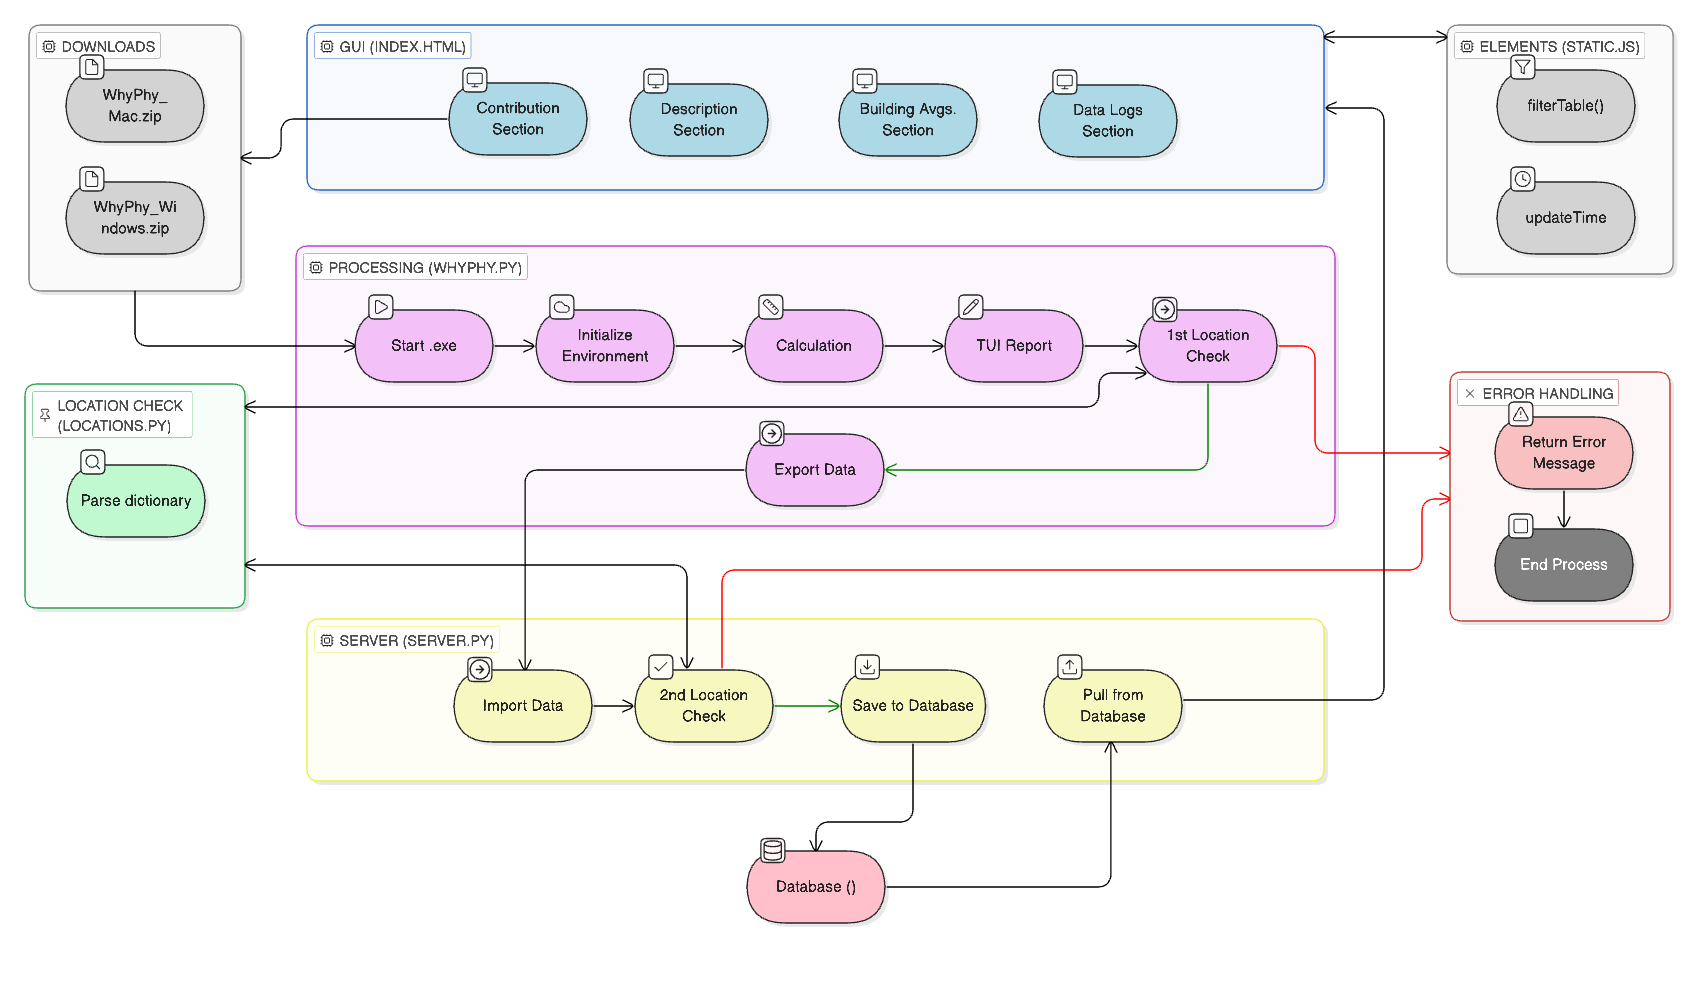
\includegraphics[width=\linewidth]{figures/diagramFigure.png}
  \caption{System Architecture. The end-to-end data processing workflow of the GetYourWhyPhy ecosystem. The pipeline initializes at the client tier, where the Python-based benchmarking script captures connection profiles. Data is serialized into a structured JSON payload and securely pushed over HTTPS to the backend logic layer FastAPI. The server commits them to the database and distributes the fresh datasets to the GetYourWhyPhy frontend for the client.}
\end{figure}

\subsection{Data Collection and Scoring Algorithm}
Benchmarks are performed using a customized implementation of speedtest-cli. This allows for the collection of five core metrics. The scoring logic prioritizes download speed and latency while penalizing high jitter and packet loss. The score is a weighted sum of five normalized sub-scores reflecting what users care about most when evaluating a connection: 

\begin{itemize}
\item {\texttt{Download Speed (35\%)}}: Throughput from the server to the client. The highest weight, as most student use cases involve consuming content like loading slides or streaming lectures.
\item {\texttt{Upload Speed (20\%)}}: Throughput from the client to the server. Important for submitting assignments or sharing data.
\item {\texttt{Latency (30\%)}}: The round-trip time for data packets. Critical for responsiveness in video calls and real-time applications.
\item {\texttt{Jitter (10\%)}}: The variation in latency over time. Measures variability in latency; inconsistent ping leads to instability.
\item {\texttt{Packet Loss (5\%)}}: Data packets that aren’t delivered. Even small fractions of packet loss significantly degrade perceived quality.
\end{itemize}

\begin{figure}[h]
  \centering
  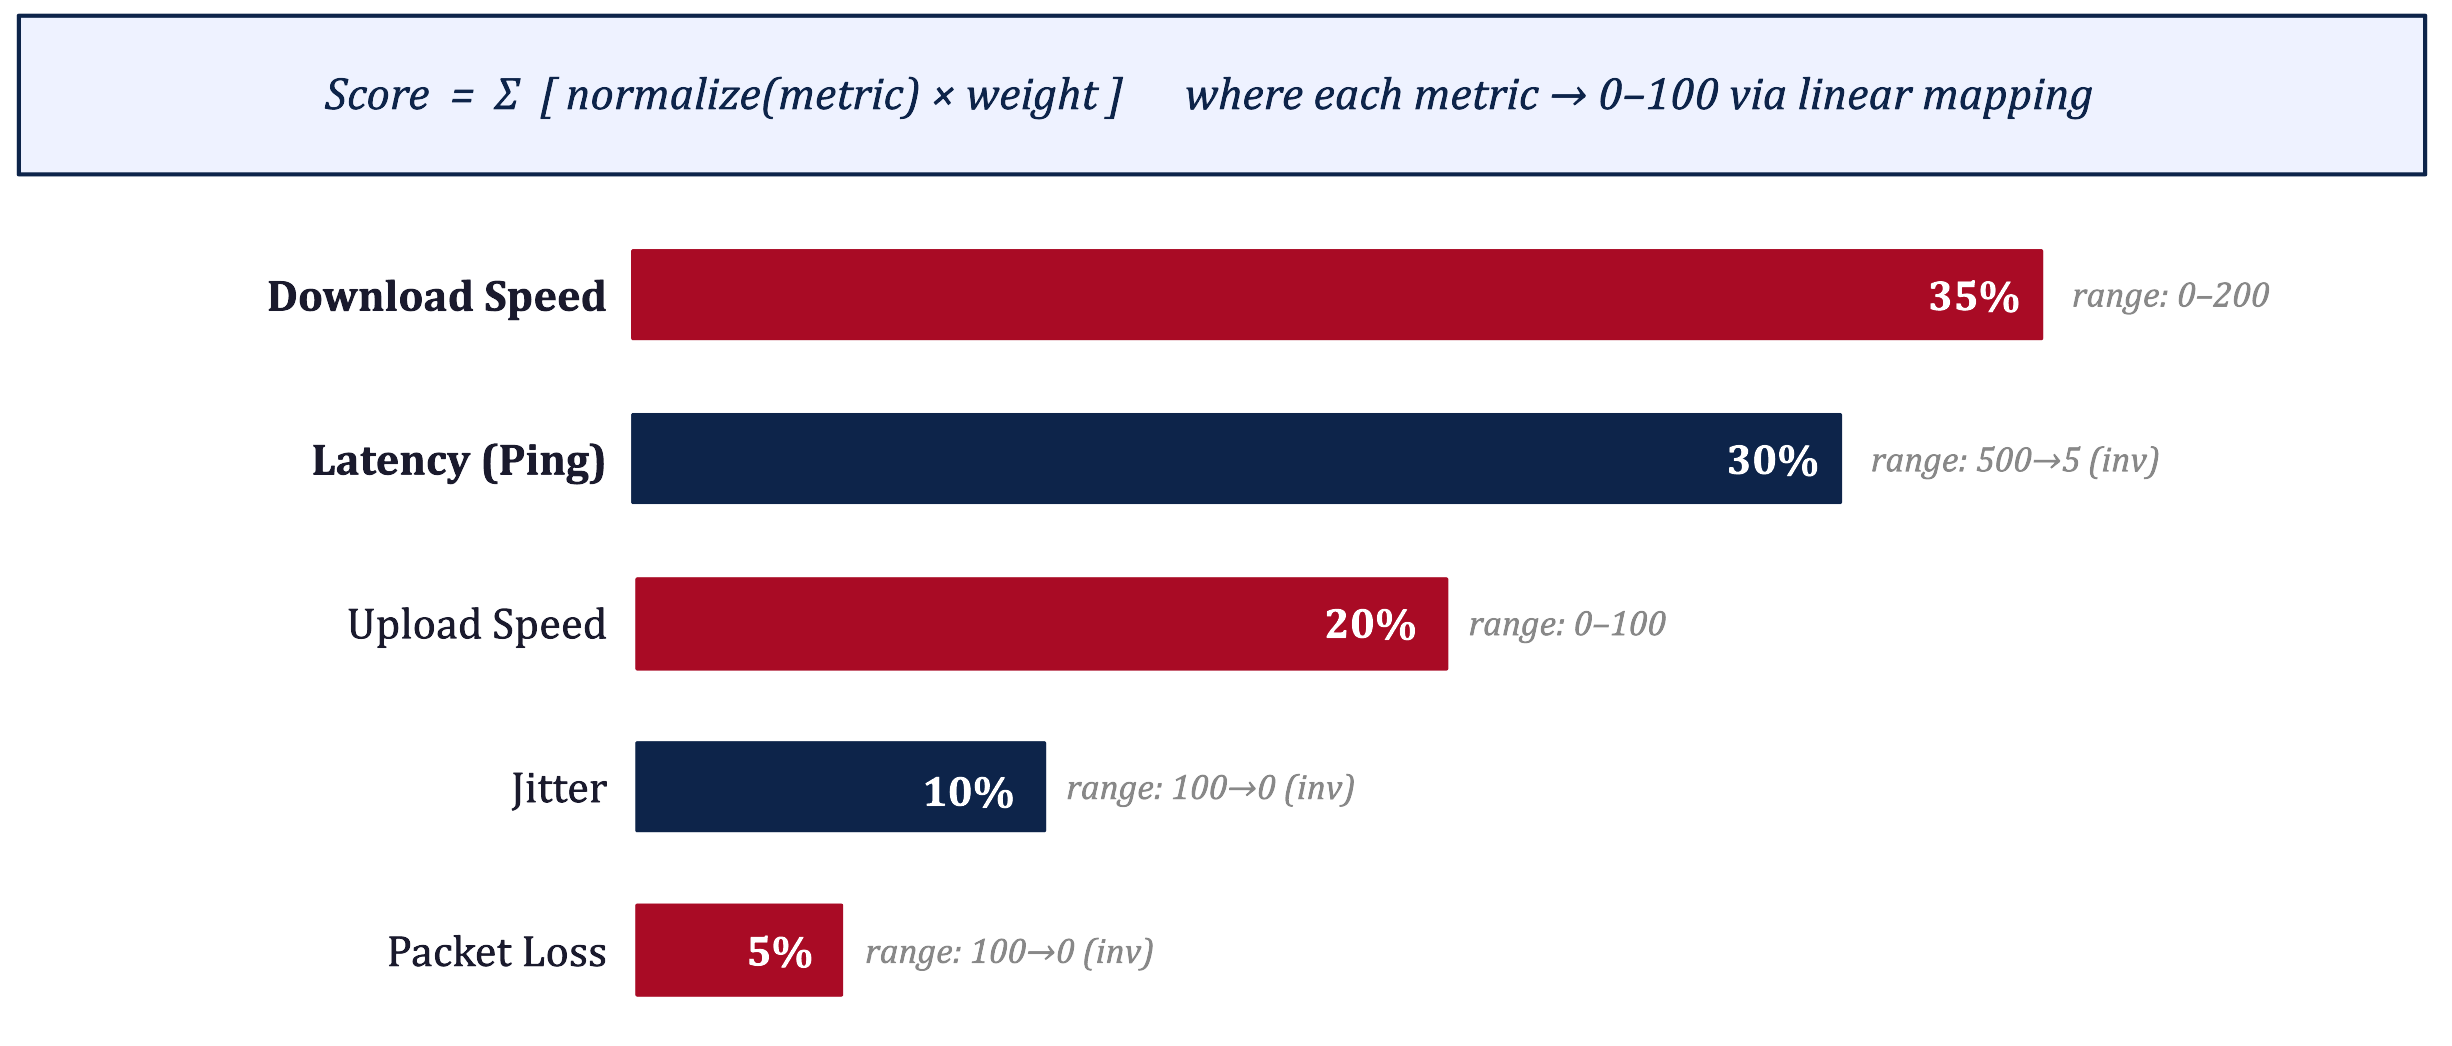
\includegraphics[width=\linewidth]{figures/normalizedScoresFigure.png}
  \caption{Normalized WhyPhy Score. This visual element shows how individual connection reports are condensed into a single numeric index. By hiding overwhelming technical terms behind a color-coded index score, non-technical users can quickly evaluate network capacity. Green profiles highlight optimal performance fields, while lower ranges signal unstable nodes full of issues.}
\end{figure}

\subsection{Linear Normalization}
Each metric is converted to a 0–100 value using linear mapping. For metrics where higher is better (Download/Upload), the score is calculated as:

$$score = clamp\left(\frac{value - floor}{ceiling - floor} \times 100, 0, 100\right)$$

For inverted metrics (Latency, Jitter, Packet Loss), the axis is flipped so that the best-case value (e.g., 5ms latency) maps to 100 . These scores then map to intuitive letter grades, where 90+ is an A+ and scores below 45 result in an F.

\begin{figure}[h]
  \centering
  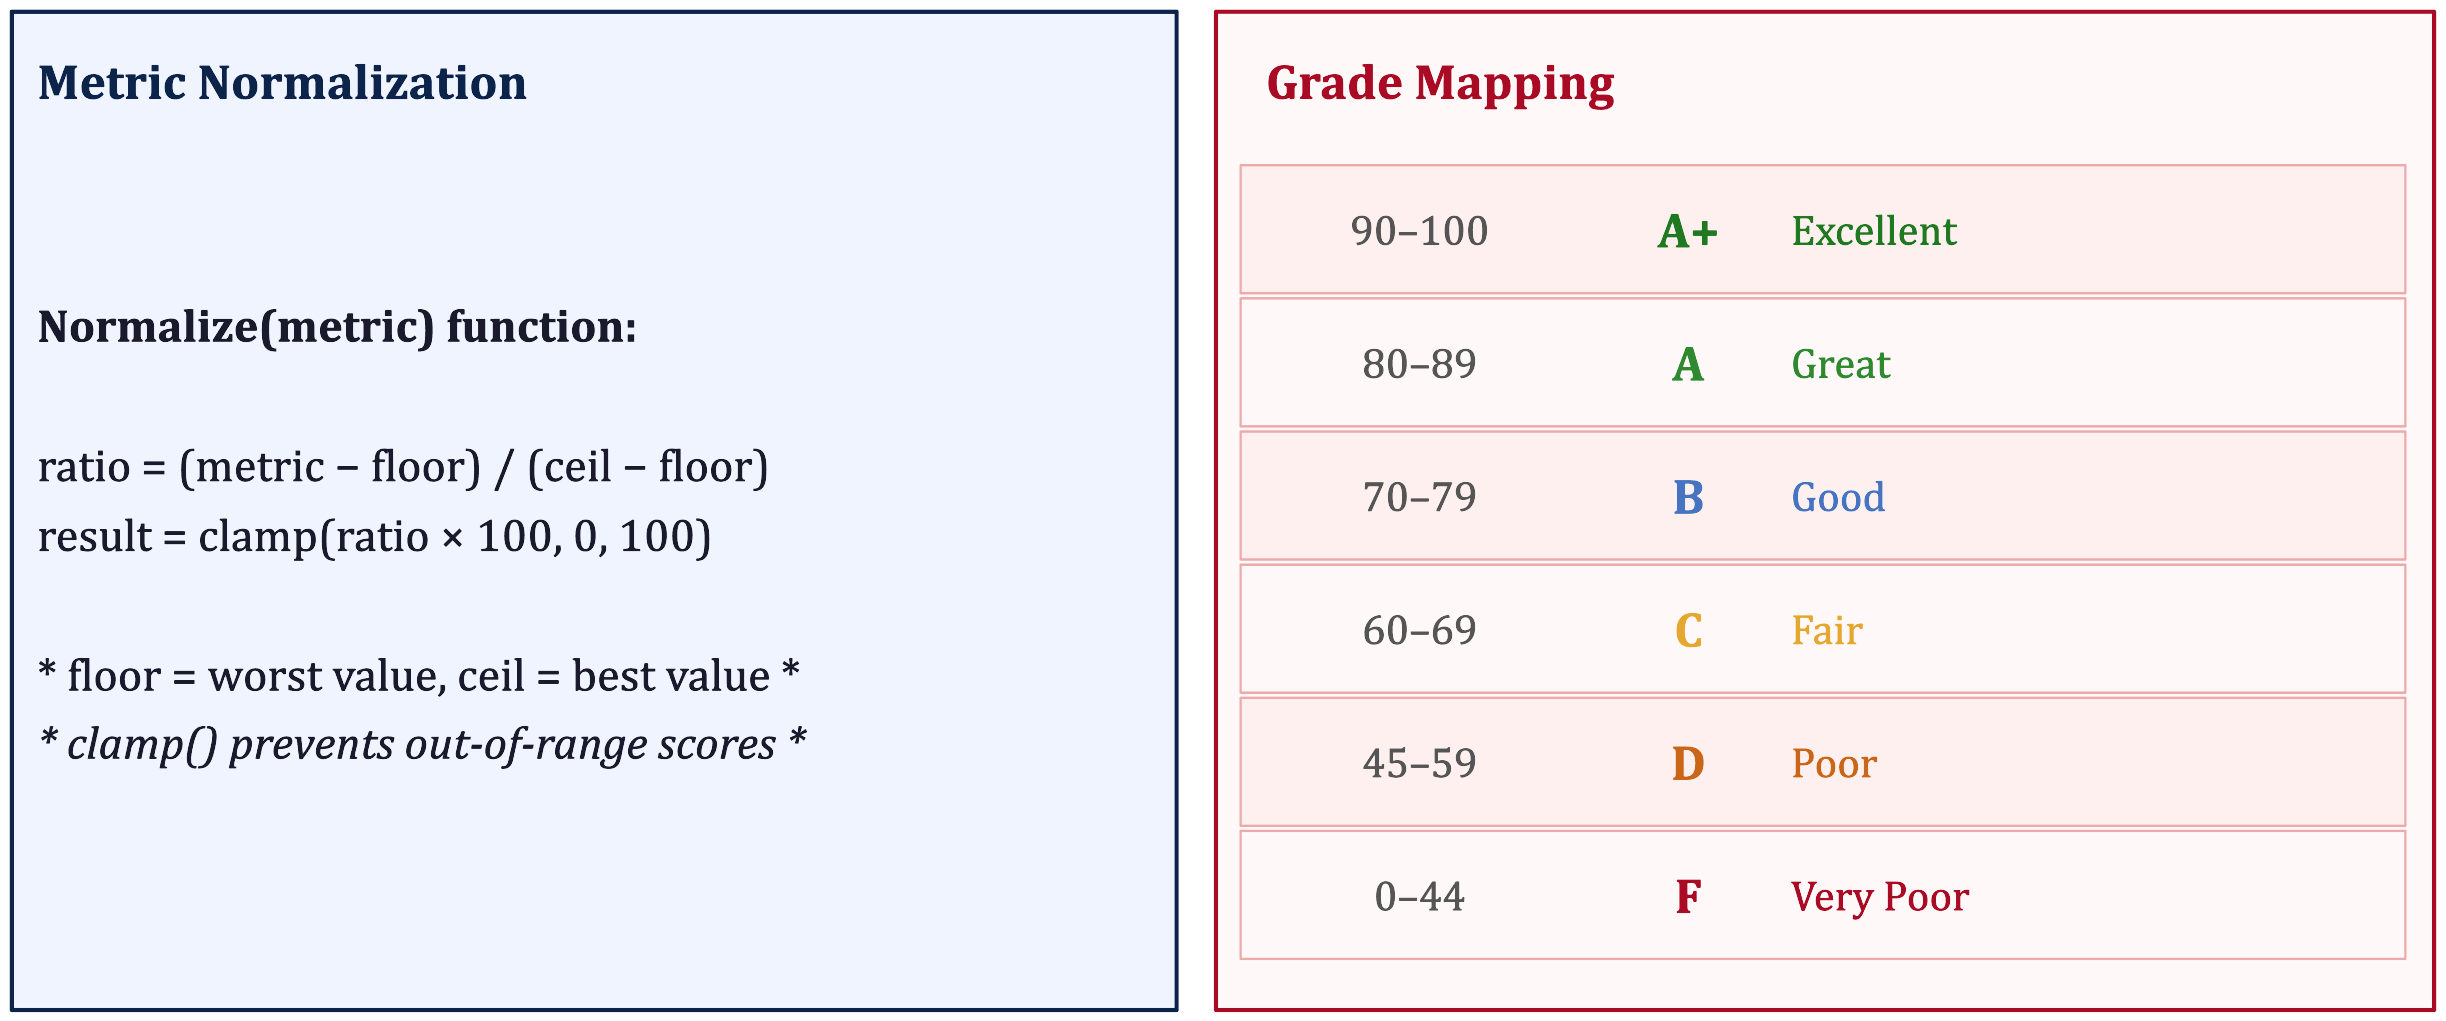
\includegraphics[width=\linewidth]{figures/normalizationCalculationFigure.png}
  \caption{Normalization Logic Flow. The mathematical translation stack used by the normalization module to convert multi-dimensional network data into a single intuitive metric. The algorithmic matrix processes highly asymmetric variables and balances them using weight coefficients. The engine actively applies exponential deduction penalties when stability bounds breaks, outputting a standardized value between 0 and 100.}
\end{figure}

\subsection{Implementing WhyPhy.py}
From the beginning, one of the primary hurdles was the multi-platform signal processing since the test needs to run on Windows, macOS, and Linux,. WhyPhy.py starts by handling the variable outputs of "netsh", "system\_profiler", and "nmcli" while manually calculating signal quality from raw dBm values for Mac users. Implementing the scoring logic introduced another layer of complexity, as the script must map diverse metrics each with a unique metric onto a unified 0–100 scale using a clamp function and weighted averages to ensure a single "jittery" metric doesn't unfairly tank the overall grade.

Finally, the FastAPI integration and TUI demanded robust error handling to manage network timeouts during the export process, all while maintaining a visually clean report using custom-drawn ASCII progress bars that dynamically reflect the health of the connection. We wanted to keep the robustness that this wifi test produced so we used pyinstaller to create a full virtual environment locally for users who ran the executable.

\subsection{Implementing server.py}
We also had to go from the TUI to a GUI, especially if we depended on this crowdsourced data for GetYourWhyPhy to function. We needed something more accessible and for this, we adopted the classical Client-Server Architecture around WhyPhy.py. After bridging this gap, running WhyPhy.py locally would allow its results to reach the wider system, both frontend and backend.

The design of the server backend was done using FastAPI because of its high performance and native asynchronous support. Now, running the WhyPhy.py locally wouldn’t just show the user a report of raw data; it packages that data into a payload using the pydantic model and then writes a JSON that can be sent as a POST request to our central server (server.py). The FastAPI backend manages the concurrent state between incoming POST requests from active network tests and GET requests from the web dashboard with the help of SQLite.

Additionally, we integrated a custom module called locations.py that acts as a 'fuzzy-matching' engine. Since users might type 'The Library' or 'Main Lib,' the logic on the server-side standardizes that input into a single database entry for the Main Library. In the list CAMPUS\_BUILDINGS, we keep all the official names of buildings and also map every possible alias to the official name to ensure our leaderboard remains clean and statistically significant.

\subsection{Implementing index.html}
Designing index.html for our GetYourWhyPhy frontend was challenging due to having to translate raw data into a readable leaderboard for the user. The first technical hurdle was implementing a dynamic search and filtering system that bridges the gap between the server.py backend and the user. Here, the UI has to responsively filter through scores and manage the Jinja2 templating logic used to render the building\_stats and logs arrays in real-time.

Also, the UI serves as the critical "hook" for community engagement since we want to endorse user engagement for crowdsourcing purposes. By using a Montserrat-based design with UA-themed red and blue color schemes, we transform the page from an abstract set of WhyPhy.py metrics into a professional "study spot finder." This emphasis on UI is vital because if the leaderboard weren't visually compelling and easy to navigate (featuring clear status badges and progress bars for building averages) students would be less likely to contribute their own reports, weakening our data set.

\section{Evaluation}
Initial testing successfully validated the core concept behind GetYourWhyPhy by demonstrating that crowdsourced wireless benchmarking can provide meaningful and actionable insight into campus Wi-Fi performance. Using our own controlled testing, crowd-sourced testing, and informal user feedback, we evaluated the usability, scalability, and effectiveness of the platform across several high-traffic locations at the University of Arizona as well as its students and faculty.

The system was tested in multiple campus buildings, including the Main Library, CESL, Gould-Simpson, the Student Union Memorial Center, and other commonly used study areas. During these tests, the benchmarking tool measured download speed, upload speed, latency, jitter, and packet loss, which were then converted into a simplified WhyPhy Score ranging from 0 to 100. The evaluation confirmed that campus Wi-Fi quality varied significantly depending on the location. We assume that the time of day and the number of users connected to the network might also be important factors.

One of the most important findings from the evaluation was that signal strength alone does not accurately represent the actual user experience. Several locations with strong wireless signal indicators still experienced high latency or unstable performance. This reinforced the project’s decision to use a weighted composite scoring model instead of relying on a single metric such as download speed. The evaluation also highlighted the effectiveness of the leaderboard-style interface shown in the presentation materials. Students enjoyed being able to quickly compare buildings and identify better study environments without needing advanced networking knowledge.

\subsection{Methods of Gathering Feedback}

To evaluate both the technical functionality and the usability of the system, the project team gathered feedback from multiple groups of users. We shared the project with professors, classmates, friends, and students who regularly relied on campus Wi-Fi for coursework and online activities. Feedback was collected immediately after these demonstrations, informal interviews, and direct observation of users interacting with the interface.

We first introduced the system in classroom environments after receiving permission from professors to present the idea and gather reactions from students. In addition to the immediate questions and feedback, we later followed up with our friends and early testers who used the software. They provided valuable insight regarding the clarity of the interface, the usefulness of the ranking system, and the practicality of the software during everyday academic activities.

The evaluation process emphasized user-centered design principles. Rather than focusing only on technical benchmarking accuracy, the project also prioritized whether students could realistically use the system to make informed decisions about where to study or attend online meetings.

\subsection{User Experience Evaluation}
The dashboard in the GetYourWhyPhy Frontend used during testing displayed ranked campus locations, Wi-Fi scores, upload and download performance, latency measurements, and recent report timestamps. Users were also able to search for specific buildings using a search bar integrated into the leaderboard system.

Overall, users responded positively to the design of the platform. Many participants stated that the leaderboard format made the information easier to understand compared to traditional networking tools such as Speedtest.net. Instead of presenting isolated measurements without context, GetYourWhyPhy provided campus-specific comparisons that directly related to student experiences.

Several users specifically praised the following features:
\begin{itemize}
\item {\texttt{}}The WhyPhy Score, which simplified complex networking metrics into a single understandable value.
\item {\texttt{}}The search functionality, which allowed users to quickly find information about a specific building.
\item {\texttt{}}The live ranking system, which encouraged comparison between study locations.
\item {\texttt{}}The campus-focused design, which provided more meaningful information than generic speed testing platforms.
\end{itemize}

The evaluation also revealed several areas for improvement. Early versions of the interface displayed every collected metric, including jitter and packet loss, directly on the main dashboard. While technically useful, many users reported that this information felt overwhelming or confusing. As a result, we refined the user interface to prioritize the overall WhyPhy Score while still retaining advanced metrics for users who wanted more detailed information.
Another issue discovered during testing involved executable setup and distribution. Some users encountered problems running the benchmarking script depending on their operating system configuration or Python environment. Even after optimizing the executable for MacOS and Windows, many permission-related hurdles remain in the way of better accessibility. These issues highlighted the importance of simplifying installation procedures and improving cross-platform compatibility in future versions of the project.

\subsection{Key Findings}
One of the most significant successes of the project was the transition from an IoT hardware-based architecture to a software-defined distributed model. Early project ideas involved ESP8266 microcontrollers and standalone sensors that would monitor Wi-Fi conditions automatically. However, the evaluation process showed that these hardware approaches introduced major challenges involving WPA2-Enterprise authentication, device management, limited memory, and physical deployment.

By transitioning to a crowdsourced software model, the system became significantly more scalable and cost effective. Instead of relying on dedicated sensors, the project leveraged devices that students already owned, including laptops and personal computers. This allowed the system to potentially scale across the entire University of Arizona campus without requiring additional infrastructure investment.

The testing process confirmed that no single metric accurately reflects user experience. For example, some locations had strong download speeds but poor latency or high jitter, which negatively affected activities such as Zoom calls or collaborative work. The WhyPhy Score successfully addressed this issue by combining multiple metrics into a single weighted score.
Crowdsourced Data Improves Transparency

The evaluation demonstrated that students valued having access to transparent, community-driven data. Many users stated that before the project existed, they relied entirely on trial and error when searching for reliable study locations. The live dashboard reduced this uncertainty by creating a public source of campus network information. Additionally, the system encouraged participation by framing the interface similarly to a leaderboard with users discussing which study spot was best and what they thought of its assigned score.

\subsection{Limitations of Evaluation}
Although the evaluation demonstrated the effectiveness of the system, several limitations remained. First, the sample size of contributors was still relatively small because testing occurred during the project development stage. A larger deployment involving hundreds of students would provide more representative data across different times, locations, and device types. Second, the benchmarking process depended on voluntary user participation. This means that some campus locations received significantly more data than others, which may have introduced bias into the rankings. Third, differences in hardware configurations between devices could affect benchmark results. Students using older laptops or weaker wireless adapters may experience different performance compared to users with newer devices. Finally, the current system still requires users to manually select or confirm their location. This introduces the possibility of human error when submitting benchmark data. Future implementations using BSSID mapping and automated location detection would improve accuracy significantly.

\subsection{Overall Evaluation Summary}
Overall, the evaluation phase confirmed that GetYourWhyPhy successfully addressed a real campus problem by transforming Wi-Fi quality from guesswork into measurable, accessible data. The combination of crowdsourced benchmarking, weighted scoring, and a simplified leaderboard interface created a system that was both technically informative and user friendly.

The project demonstrated that software-defined monitoring can serve as a practical alternative to expensive hardware-based network infrastructure. User feedback strongly supported the idea of expanding the platform further, particularly through automated mapping, passive background testing, and predictive analytics.

\begin{figure}[h]
  \centering
  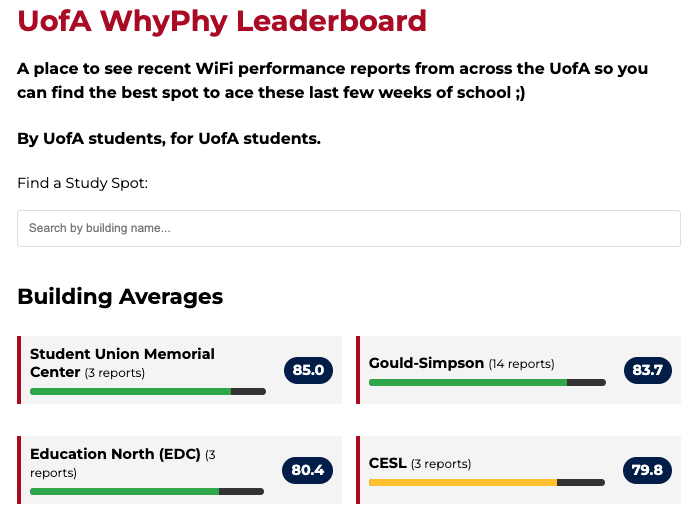
\includegraphics[width=\linewidth]{figures/lookupAveragesBuildingsReportsFigure.png}
  \caption{Building Lookup and Trends Dashboard. The diagnostic component of the web application used to track network behavior across different campus areas. The interface groups individual test logs by building profile, allowing users to isolate network trends between buildings.}
\end{figure}

\section{Future Work and Discussion}

GetYourWhyPhy provides a foundation for smarter campus infrastructure planning. Future development will focus on:

\begin{itemize}
\item {\texttt{Automated Mapping}}: Utilizing BSSID data to automatically identify buildings without requiring user input.
\item {\texttt{Passive Testing}}: Background monitoring to detect connectivity drops in real-time.
\item {\texttt{Predictive Analytics}}: Using historical trends to forecast network congestion during peak hours.
\end{itemize}

To better evaluate the effectiveness of the system, we would conduct a series of controlled tests across five major campus lo- cations over a two-week period. To ensure the results and evaluation is robust, the tests would be done so through a standardized laptop configuration (Intel i7, 16GB RAM) running the GetYour- WhyPhy CLI tool. We targeted three high-density locations (Main Library, CESL, Student Union) and two low-density locations (Enke Drive study areas). Furthermore, each location would be tested at three different intervals; 9:00 AM (low load), 1:00 PM (peak load), and 8:00 PM (medium load).

The current iteration of GetYourWhyPhy relies on manual user input for building identification. A primary limitation is the potential for human error when selecting a location from the drop-down menu. To address this, future work will integrate BSSID (Basic Service Set Identifier) mapping. By correlating the unique WhyPhy MAC address of the local Wi-Fi access point with a campus data- base, the system could automatically identify the user’s building and room number, significantly increasing data accuracy.

Furthermore, we plan to implement "Passive Background Testing." This would allow the software to monitor connectivity drops in the background without requiring the user to manually trigger a test. This "IoT-lite" approach would provide a much higher density of data, allowing for the creation of heatmaps that track network health in real-time across the entire campus.

\section{Conclusion}
GetYourWhyPhy addresses the critical need for transparent campus network performance data. By shifting from a hardware-centric monitoring model to a crowdsourced, software-defined benchmarking system, we have created a scalable tool that empowers students to make data-driven decisions about their study environments. Our evaluation confirms that simple throughput metrics are insufficient for characterizing network quality; instead, a multi-metric normalized score provides a more accurate representation of academic network utility.

\section{Acknowledgment}
\begin{itemize}
\item {\texttt{}}Aleco Dominguez: Authored Section 1 (Introduction), Section 3 (Design and Methodology), Sections 4.1, 4.4, 4.5, 4.6 (Implementation and Scoring) and Section 6 (Future Work). Attempted IoT Ghost approach, managed GitHub repository and coded the server-side logic and frontend.
\item {\texttt{}}Jaden Beil: Authored Section 4 (Implementation and Scoring) and Section 7 (Conclusion). Research in WiFi testing, coded the main test using the speed-cli library, edited the demo video, conducted field testing.
\item {\texttt{}}RJ Edwards: Authored Abstract, Section 2 (Related Work), Section 5 (Evaluation), and formatted the final manuscript. Outreach for crowdsourcing, developed frontend visualization components, worked on client-server architecture.
\item {\texttt{}}AI Disclosure: The authors utilized a large language model (Gemini) to assist in structuring the documentation according to the ACM double-column format and to expand on the technical descriptions of the normalization algorithm and evaluation results. All AI-generated content was reviewed, edited, and verified against the actual repository code and project outcomes by us.
\end{itemize}


%%
%% The next two lines define the bibliography style to be used, and
%% the bibliography file.
\nocite{*}
\bibliographystyle{ACM-Reference-Format}
\bibliography{references}

\end{document}
\endinput
%%
%% End of file `sample-sigconf-authordraft.tex'.
